\begin{frame}{VOISING からの落下点は通年で海上}{結果：北海道の落下位置}
  \begin{columns}[T]
    \begin{column}{0.38\textwidth}
      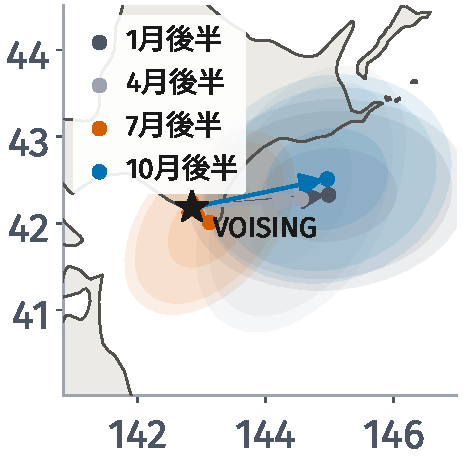
\includegraphics[width=\linewidth,height=140pt,keepaspectratio]{S_voising_landing_seasons.pdf}
    \end{column}
    \begin{column}{0.60\textwidth}
      \begin{columns}[T]
        \begin{column}{0.56\textwidth}
          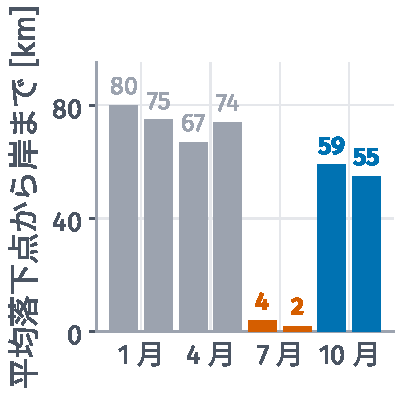
\includegraphics[width=\linewidth,height=100pt,keepaspectratio]{S_offshore_bars.pdf}
        \end{column}
        \begin{column}{0.42\textwidth}
          \vskip 1mm
          \midnum[wcOrange]{2--4}{km}{7 月だけ岸のすぐそば}
          \vskip 3mm
          \midnum{55--80}{km}{他の季節は沖。船が要る}
        \end{column}
      \end{columns}
      \vskip 1mm
      \sub{変わるのは「海か陸か」ではなく\kw{岸からの距離}。\\地点の性質。内陸から上げれば陸に落ちる。}
    \end{column}
  \end{columns}
  \srcline{楕円は 50 / 90 / 95 \%、各月の後半ビン。地点固有の結果、道北・道東には使わない}
\end{frame}
